% \section*{About the Authors}

% % TODO: Define \bio command!


% % \bio{bio-images/evans.png}
% % Theodore Evans is a Ph.D. Candidate at the DAI-Labor at the TU Berlin. He received his M.Phys. degree in Physics from the University of Manchester. He is currently supervised by Prof. Dr. Dr. hc Sahin Albayrak. His research interests lie in representation learning and cross-disciplinary approaches to explainable AI-assistance for digital pathology.
% % \endbio

%  \begin{wrapfigure}{l}{25mm} 
%     
\includegraphics[width=1in,height=1.25in,clip,keepaspectratio]{bio-images/evans.JPG}
%   \end{wrapfigure}\par
%   \textbf{Theodore Evans} is a Ph.D. Candidate at the DAI-Labor at the TU Berlin. He received his M.Phys. degree in Physics from the University of Manchester. He is currently supervised by Prof. Dr. Dr. hc Sahin Albayrak. His research interests lie in representation learning and cross-disciplinary approaches to explainable AI-assistance for digital pathology.\par

%\bio{bio-images/retzlaff.jpg}
%Carl Orge Retzlaff is research assistant and PhD student at the DAI-Labor at TU Berlin. He previously obtained a B. Sc. and an M. Sc. degree in Technical Communication, an interdisciplinary study program combining communication science and linguistics with computer science at RWTH Aachen University. His research interests are agent-based modelling and a combination of Human Computer Interaction theories with explainable AI approaches.
%\endbio

 \begin{wrapfigure}{l}{25mm} 
    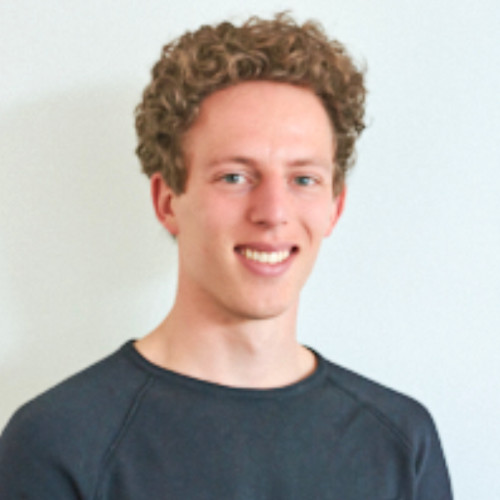
\includegraphics[width=1in,height=1.25in,clip,keepaspectratio]{bio-images/retzlaff.jpg}
  \end{wrapfigure}\par
  \textbf{Carl Orge Retzlaff} is research assistant and PhD student at the DAI-Labor at TU Berlin. He obtained a B. Sc. and an M. Sc. degree in Technical Communication, an interdisciplinary study program combining communication science and linguistics with computer science at RWTH Aachen University. His research interests are agent-based modelling and a combination of Human Computer Interaction theories with explainable AI approaches.\par

%\bio{bio-images/geissler.jpg}
%MChristian Geißler is PhD student and leader of the artificial intelligence and machine learning group at the DAI-Labor at the TU Berlin. He obtained a B.Sc. and M.Sc. in Computer Engineering with a focus on cognitive systems. His research interests are optimization, algorithm selection, automated machine learning and applied explainable artificial intelligence.
%\endbio

 \begin{wrapfigure}{l}{25mm} 
    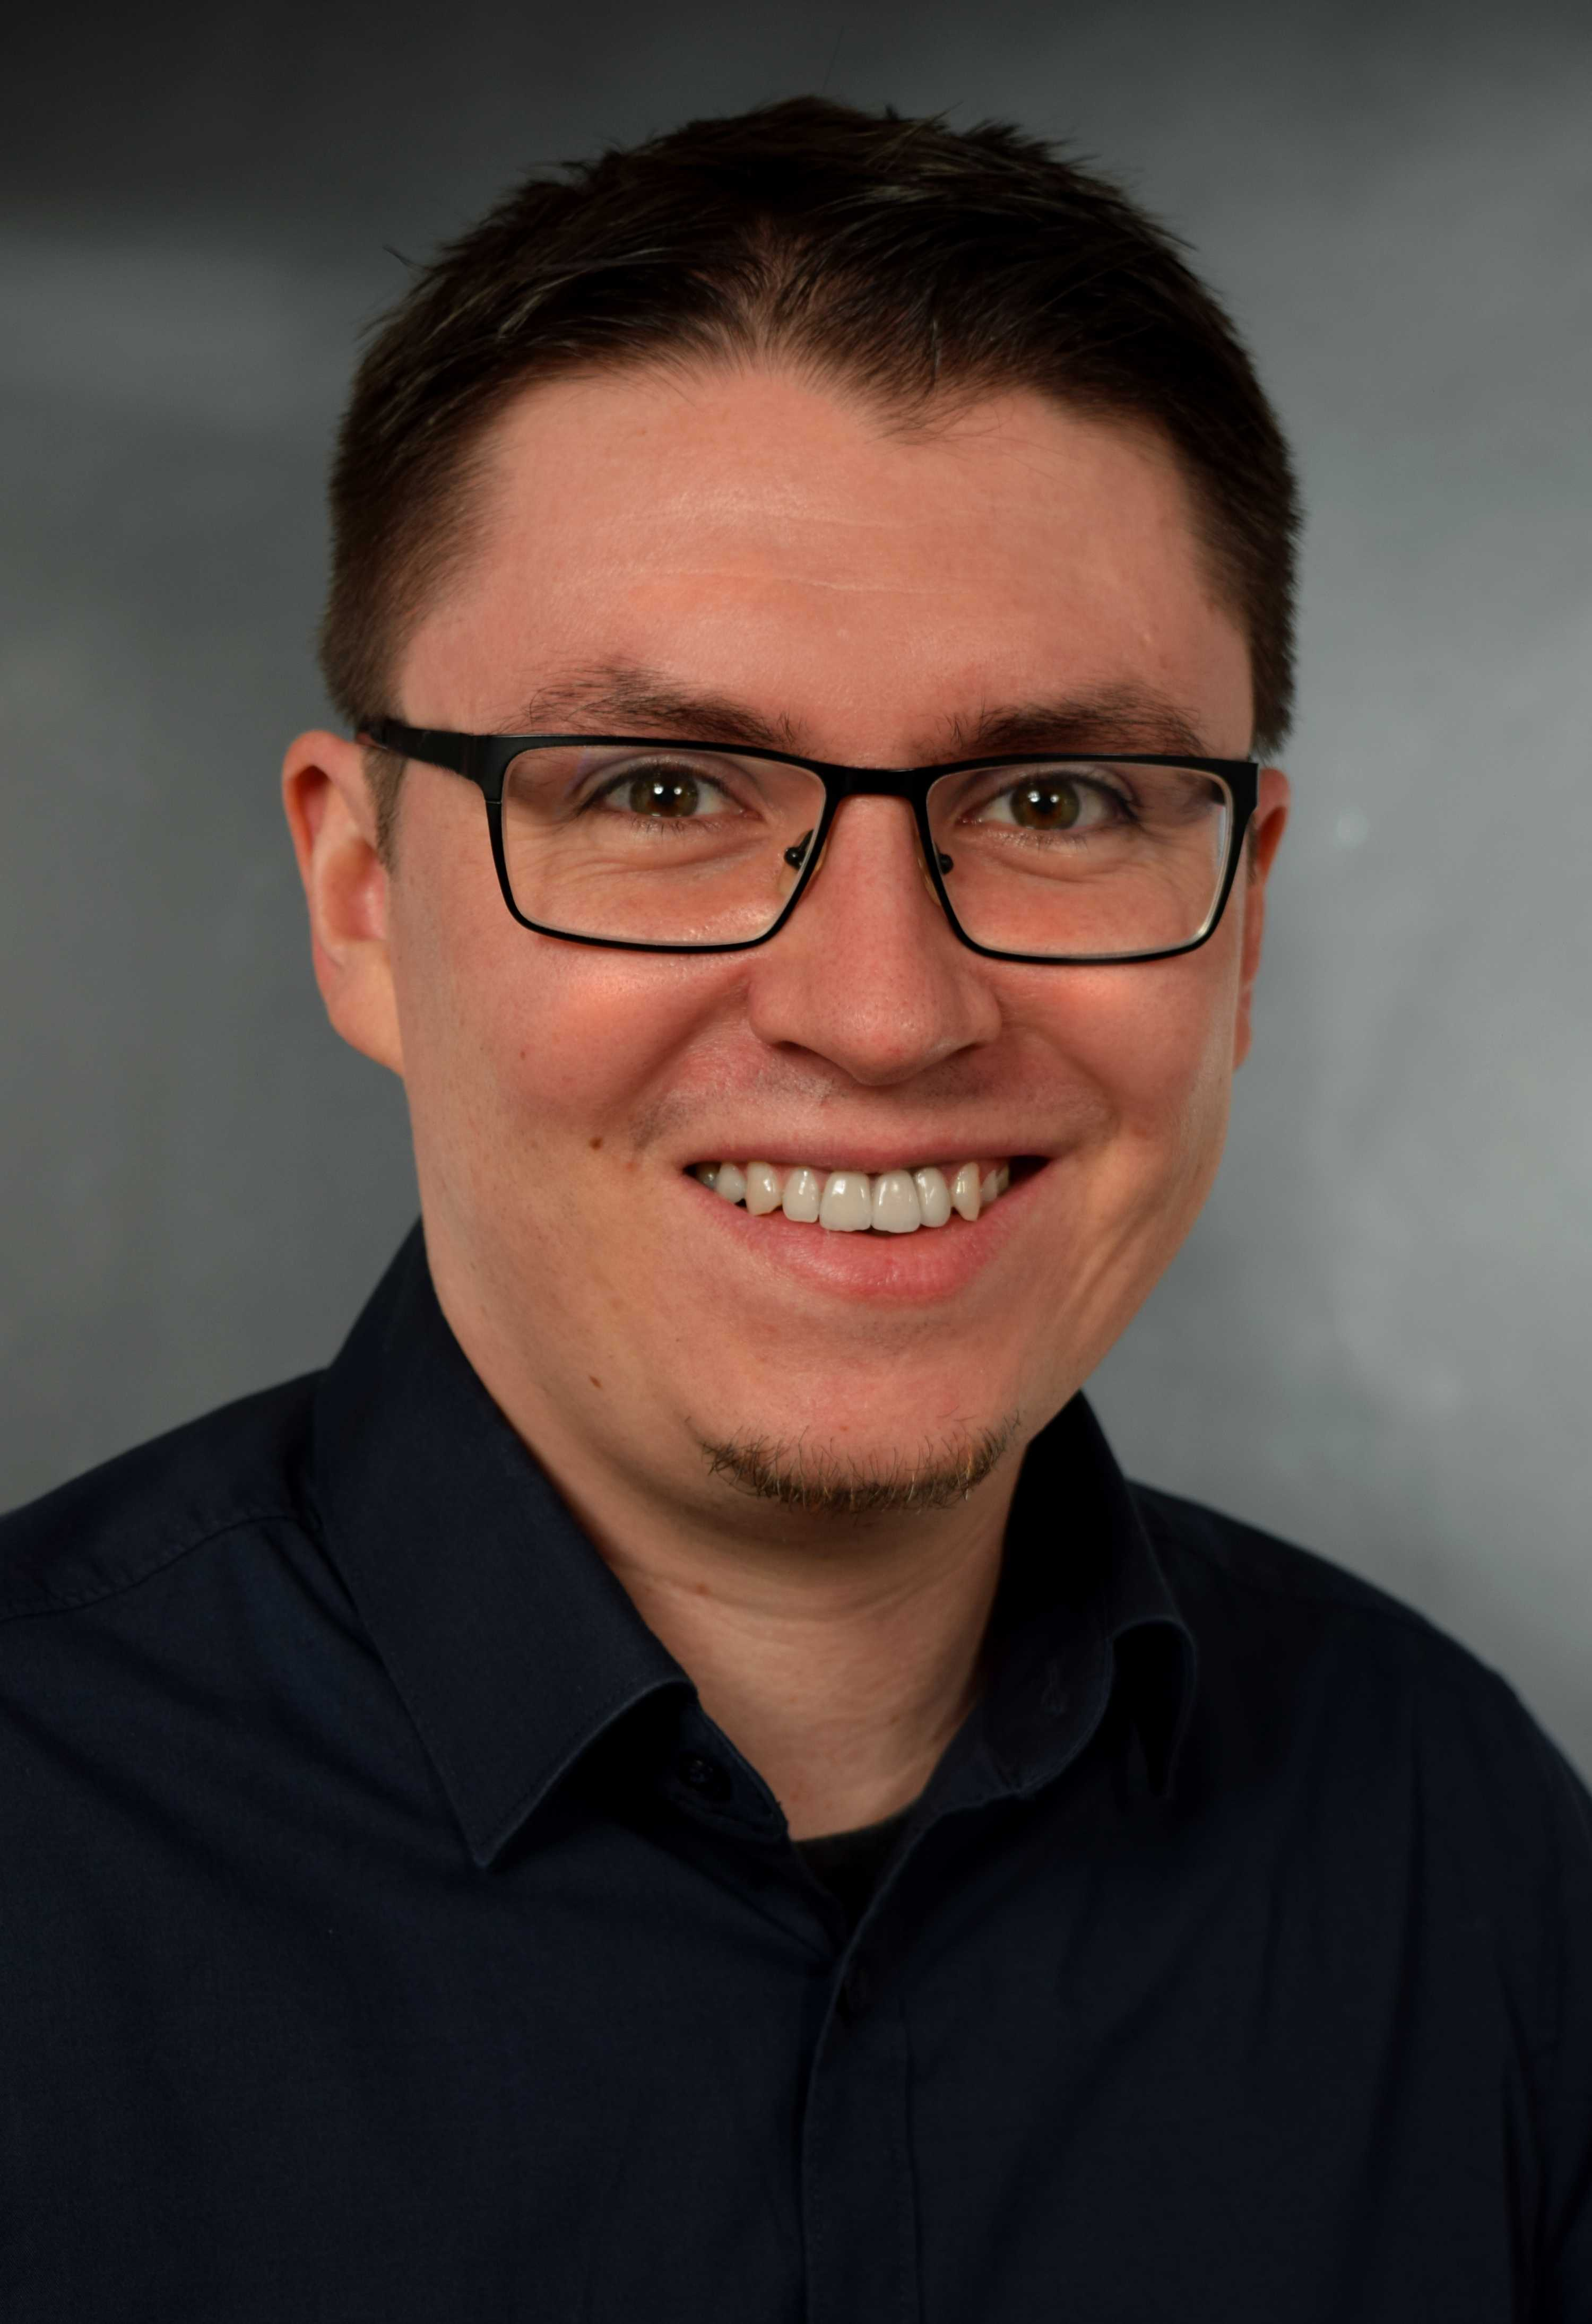
\includegraphics[width=1in,height=1.25in,clip,keepaspectratio]{bio-images/geissler.jpg}
  \end{wrapfigure}\par
  \textbf{ Christian Geißler} is PhD student and leader of the artificial intelligence and machine learning group at the DAI-Labor at the TU Berlin. He obtained a B.Sc. and M.Sc. in Computer Engineering with a focus on cognitive systems. His research interests are optimization, algorithm selection, automated machine learning and applied explainable artificial intelligence.\par

%\bio{bio-images/kargl.jpg}
%Michaela Kargl works as a research associate at the Diagnostics and Research Institute of Pathology at the Medical University Graz. She has got a degree in electrical engineering and in  information and computer engineering from Graz University of Technology. Her main research interests lie in user research, UX and usability.
%\endbio

 \begin{wrapfigure}{l}{25mm} 
    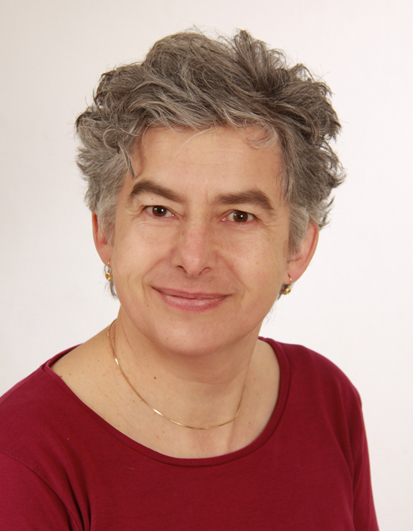
\includegraphics[width=1in,height=1.25in,clip,keepaspectratio]{bio-images/kargl.jpg}
  \end{wrapfigure}\par
  \textbf{Michaela Kargl} works as a research associate at the Diagnostics and Research Institute of Pathology at the Medical University Graz. She has got a degree in electrical engineering and in  information and computer engineering from Graz University of Technology. Her main research interests lie in user research, UX and usability.\par

% \bio{bio-images/plass.jpg}
% Markus Plass is a member of the Information Science and Machine Learning Group at the Diagnostic and Research Center for Molecular BioMedicine at the Medical University Graz, Austria. He holds a B. Sc. and  a M. Sc. degree in Biomedical Engineering from the Technical University Graz. At the university institute, he is in charge of digital pathology. His main research interests lie in digital pathology, machine learning and process optimization of digital work flows.
% \endbio
  
  \begin{wrapfigure}{l}{25mm} 
    
\includegraphics[width=1in,height=1.25in,clip,keepaspectratio]{bio-images/dummy.jpg}
  \end{wrapfigure}\par
  \textbf{Markus Plass} is a member of the Information Science and Machine Learning Group at the Diagnostic and Research Center for Molecular BioMedicine at the Medical University Graz, Austria. He holds a B. Sc. and  a M. Sc. degree in Biomedical Engineering from the Technical University Graz. At the university institute, he is in charge of digital pathology. His main research interests lie in digital pathology, machine learning and process optimization of digital work flows.\par

% \bio{bio-images/mueller.jpg}
%  
% \endbio

 \begin{wrapfigure}{l}{25mm} 
    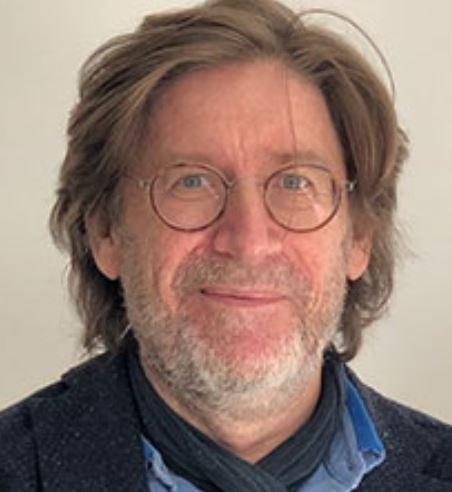
\includegraphics[width=1in,height=1.25in,clip,keepaspectratio]{bio-images/mueller.JPG}
  \end{wrapfigure}\par
  \textbf{Heimo Mueller} is head of the Information Sciences and Machine Learning Group at the Diagnostic and Research Center for Molecular BioMedicine at the Medical University Graz, Austria, and he is scientific officer at the BBMRI-ERIC. He received his PhD in Mathematics from Vienna University of Technology with a work on data space semantics. Heimos main research interests are in digital pathology and AI applications.\par


%\bio{bio-images/kiehl.jpg}
%MTim-Rasmus Kiehl is a neuropathologist with a medical degree from the University of Lübeck (1998). After a research fellowship in neurogenetics at Cedars-Sinai Medical Center, Los Angeles, CA (1999-2001), he pursued residency training in Anatomic Pathology (Stanford Univ.) and Neuropathology (MGH/Harvard Univ.). He then took a staff position at University Health Network (UHN) in Toronto, Canada from 2006-2017 (academic appointment: Univ. of Toronto). He subsequently joined Fraunhofer MEVIS, Bremen, Germany as a visiting scientist. Since 2019 he has been at Charité Universitätsmedizin Berlin as a researcher to support the project EMPAIA (EcosysteM for Pathology Diagnostics with AI Assistance). 
%\endbio

 \begin{wrapfigure}{l}{25mm} 
    
\includegraphics[width=1in,height=1.25in,clip,keepaspectratio]{bio-images/kiehl.jpg}
  \end{wrapfigure}\par
  \textbf{Tim-Rasmus Kiehl} is a neuropathologist with a medical degree from the University of Lübeck (1998). After a research fellowship in neurogenetics at Cedars-Sinai Medical Center, Los Angeles, CA (1999-2001), he pursued residency training in Anatomic Pathology (Stanford Univ.) and Neuropathology (MGH/Harvard Univ.). He then took a staff position at University Health Network (UHN) in Toronto, Canada from 2006-2017 (academic appointment: Univ. of Toronto). He subsequently joined Fraunhofer MEVIS, Bremen, Germany as a visiting scientist. Since 2019 he has been at Charité Universitätsmedizin Berlin as a researcher to support the project EMPAIA (EcosysteM for Pathology Diagnostics with AI Assistance).\par
  
  \begin{wrapfigure}{l}{25mm} 
    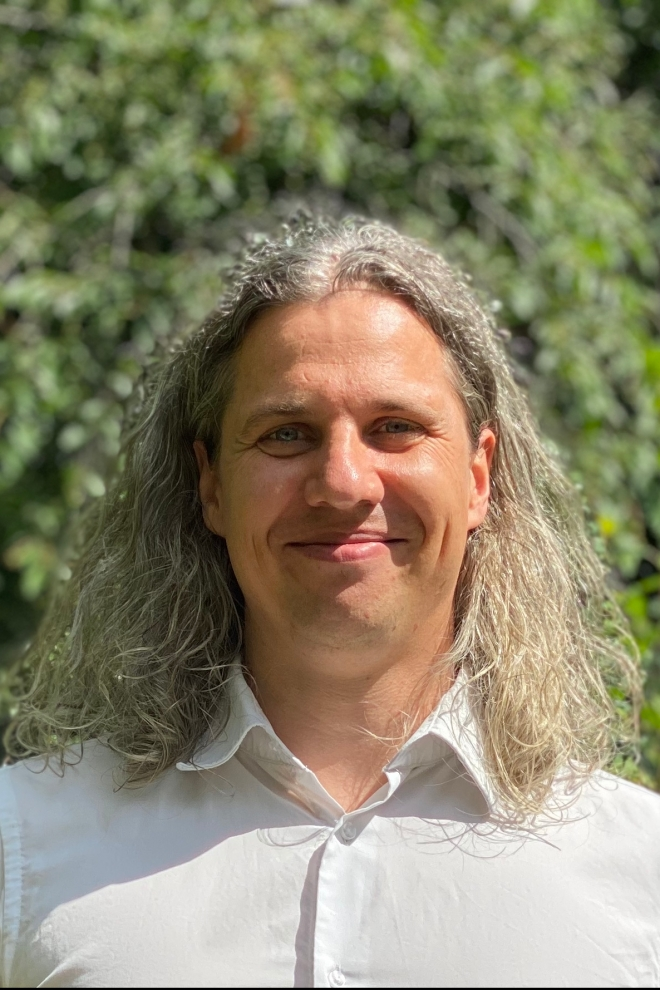
\includegraphics[width=1in,height=1.25in,clip,keepaspectratio]{bio-images/zerbe.jpg}
  \end{wrapfigure}\par
  \textbf{Norman Zerbe} is researcher at Charité Universitätsmedizin Berlin as a researcher to support the project EMPAIA (EcosysteM for Pathology Diagnostics with AI Assistance).\par

% \bio{bio-images/holzinger.jpg}
% Andreas Holzinger is Visiting Professor for explainable AI at the University of Alberta, Canada since 2019 and head of the Human-Centered AI Lab at the Medical University Graz, Austria. He received his PhD in cognitive science from Graz University and his second PhD in computer science from Graz University of Technology. Andreas was elected ordinary member in the Academia Europaea, the European Academy of Sciences in the section Informatics, for his pioneering work in interactive machine learning with the human-in-the-loop. Andreas is full member of the European Lab for Learning and Intelligent Systems.
% \endbio

 \begin{wrapfigure}{l}{25mm} 
    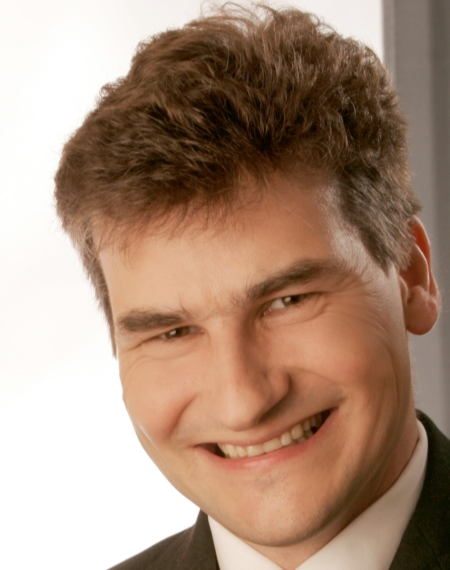
\includegraphics[width=1in,height=1.25in,clip,keepaspectratio]{bio-images/holzinger.jpg}
  \end{wrapfigure}\par
  \textbf{Andreas Holzinger} is Visiting Professor for explainable AI at the University of Alberta, Canada since 2019 and head of the Human-Centered AI Lab at the Medical University Graz, Austria. He received his PhD in cognitive science from Graz University and his second PhD in computer science from Graz University of Technology. Andreas was elected ordinary member in the Academia Europaea, the European Academy of Sciences in the section Informatics, for his pioneering work in interactive machine learning with the human-in-the-loop. Andreas is full member of the European Lab for Learning and Intelligent Systems.\par
